Az egyik legfontosabb része a projektnek a UI, amelynek megtervezésére a Figma segédprogramot használtuk, amelyben megépítettük az első elképzelésünket a felületekről. Ezt a wireframe-et követve már egyszerűbb volt a fejlesztés. Munka közben jöttek jobb ötletek is, mint a kezdeti, így nem minden egyezik a végső termékkel, de iránymutatásnak megfelelt:

\begin{figure}[H]
  
\includegraphics[width=\textwidth]{figures/ui-mobile.png}
  \caption{A mobilalkalmazás terve}
  \label{fig:ui-mobile}
\end{figure}

\begin{multicols*}{2}
  \begin{figure}[H]
    \centering
    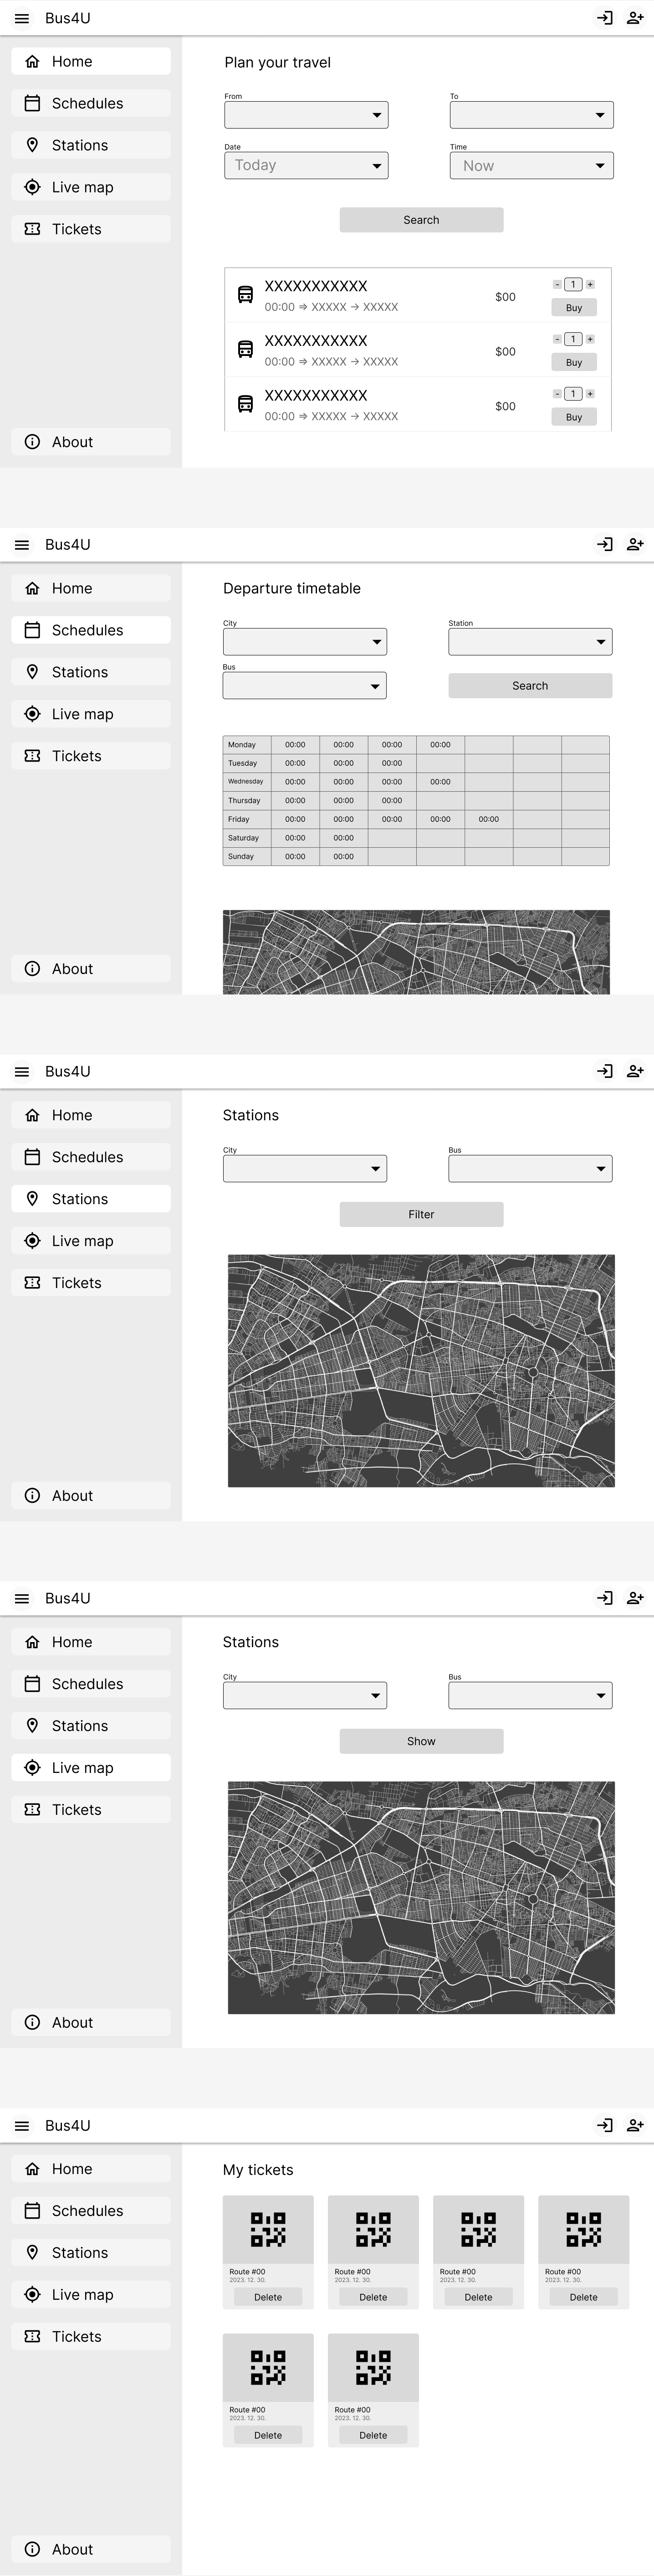
\includegraphics[height=23cm]{figures/ui-web.png}
    \caption{A felhasználói weboldal terve}
    \label{fig:ui-web}
  \end{figure}
  \begin{figure}[H]
    \centering
    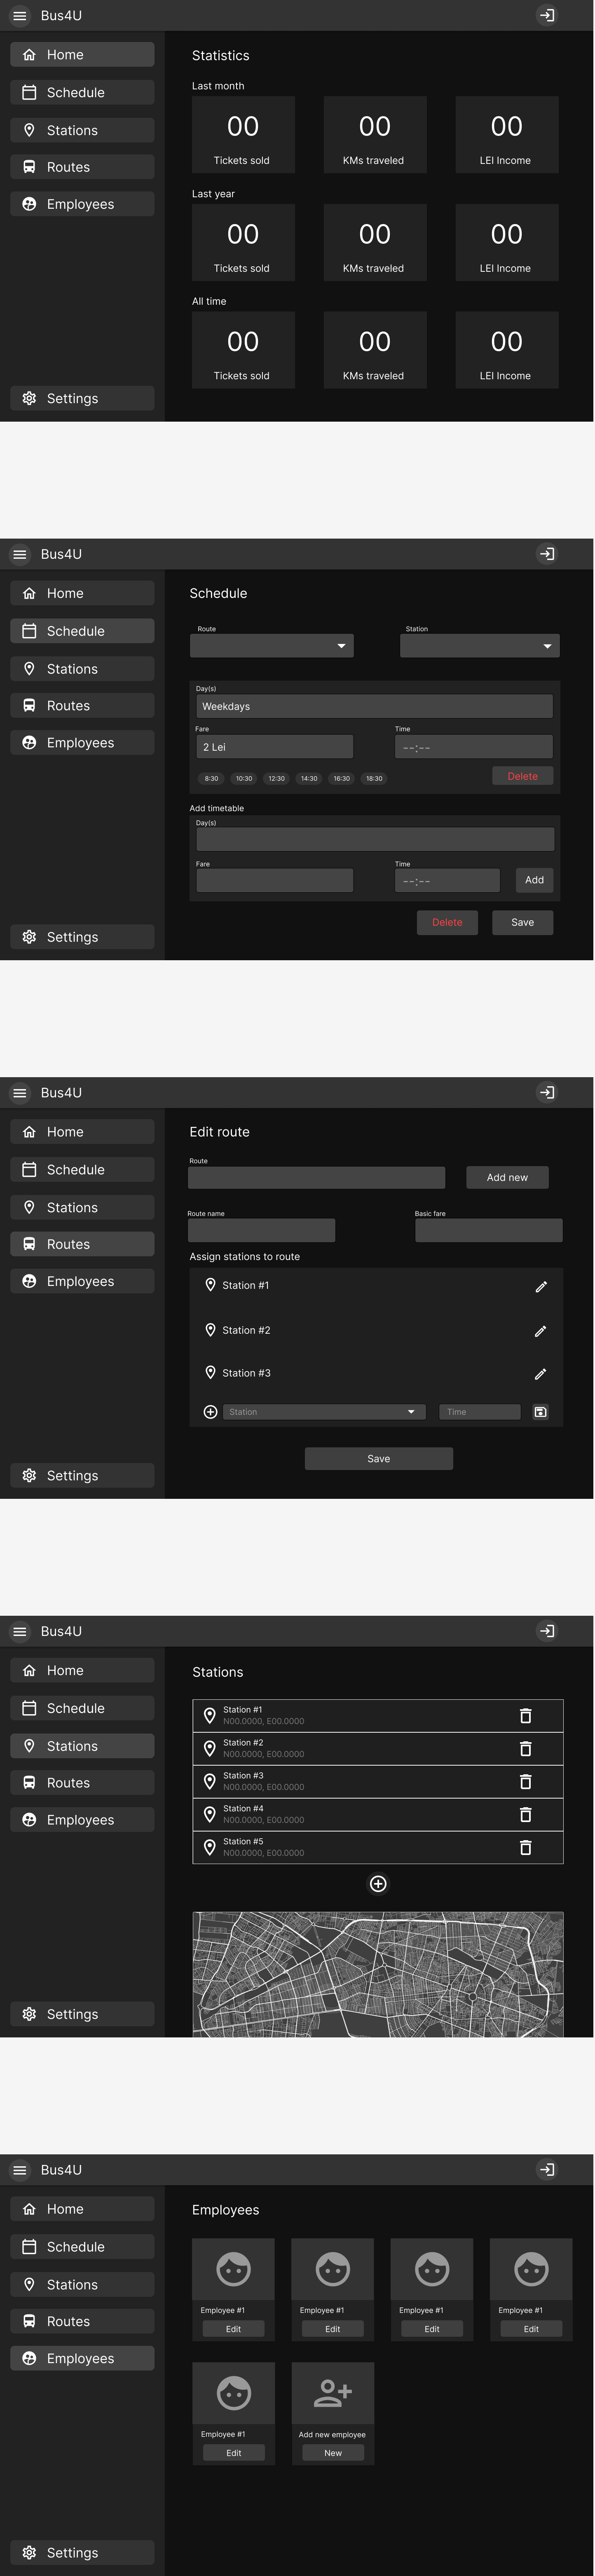
\includegraphics[height=23cm]{figures/ui-admin.png}
    \caption{Az admin weboldal terve}
    \label{fig:ui-admin}
  \end{figure}
\end{multicols*}